\documentclass{article}
\usepackage[utf8]{inputenc}
\usepackage{amsmath}
\usepackage{cite}
\usepackage[letterpaper,top=1cm,bottom=2cm,left=1.5cm,right=1.5cm]{geometry}
\usepackage{wrapfig}
\usepackage{graphicx}
\usepackage{caption}  % Paquete para personalizar captions
\captionsetup[figure]{labelfont=bf, labelsep=colon, name=Imagen} % Customiza las captions

\title{Consulta: Las Tres Formas de Cargar un Cuerpo}
\author{Ariel Alejandro Calderón}
\date{Septiembre 2024}

\begin{document}

\maketitle

\section{Carga por Fricción}


\begin{wrapfigure}{r}{0.4\textwidth}
    \centering
    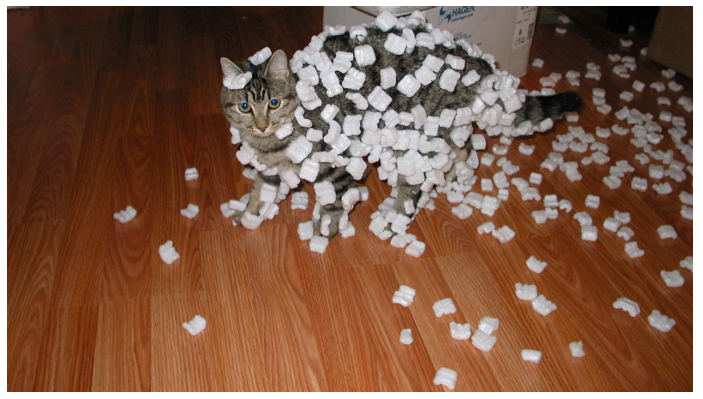
\includegraphics[width=0.33\textwidth]{./public/friccion.png}
    \caption{Carga por fricción.}
\end{wrapfigure}

La carga por fricción ocurre cuando dos cuerpos diferentes se frotan entre sí. Durante este proceso, los electrones, que son las partículas subatómicas responsables de la carga negativa, pueden transferirse de un cuerpo al otro. Este fenómeno depende de la afinidad de los materiales por los electrones. 

Cuando un material tiene mayor tendencia a ganar electrones, se carga negativamente, mientras que el material que pierde electrones se carga positivamente. Un ejemplo clásico es el frotamiento de un globo contra el cabello: el globo se carga negativamente al ganar electrones, mientras que el cabello se carga positivamente al perderlos.

Este tipo de carga es común en materiales aislantes, ya que los electrones no pueden moverse fácilmente a través de ellos.

\section{Carga por Contacto}
La carga por contacto implica que un cuerpo cargado toque físicamente a otro cuerpo neutro. Cuando esto ocurre, los electrones pueden transferirse del cuerpo cargado al neutro. El resultado es que ambos cuerpos terminan con la misma clase de carga, ya que los electrones tienden a distribuirse hasta que ambos cuerpos alcanzan un estado de equilibrio eléctrico.

Por ejemplo, si un objeto positivamente cargado toca un cuerpo neutro, algunos electrones del cuerpo neutro serán transferidos hacia el cuerpo cargado para equilibrar la carga, y ambos cuerpos se cargarán positivamente. Este fenómeno ocurre debido a la tendencia de las cargas de redistribuirse hasta que el potencial eléctrico sea igual en ambos cuerpos.

\section{Carga por Inducción}
La carga por inducción es un proceso en el cual un cuerpo cargado induce una redistribución de cargas en otro cuerpo sin necesidad de contacto directo. Cuando un cuerpo cargado se aproxima a un cuerpo neutro, las cargas dentro de este último se redistribuyen: las cargas de signo contrario al cuerpo cargado se acercan a la superficie más cercana, mientras que las cargas de igual signo se alejan.

Para cargar un cuerpo por inducción, es necesario conectar el cuerpo neutro a tierra mientras se encuentra en presencia del cuerpo cargado. Esto permite que las cargas de un signo escapen, dejando al cuerpo cargado con una carga opuesta al cuerpo que lo indujo. Al desconectar la tierra, el cuerpo se mantiene cargado.

Un ejemplo de carga por inducción es cuando acercamos un objeto cargado negativamente a una esfera metálica. Las cargas positivas se agrupan en el lado más cercano al objeto cargado, y si conectamos la esfera a tierra, los electrones en exceso abandonan la esfera, dejándola cargada positivamente.

\section*{Bibliografía}
\begin{itemize}
    \item Tipler, P. A., \& Mosca, G. (2008). \textit{Física para la ciencia y la tecnología}. Volumen 2. Reverté.
    \item Serway, R. A., \& Jewett, J. W. (2014). \textit{Física para ciencias e ingeniería}. Cengage Learning.
    \item Young, H. D., \& Freedman, R. A. (2012). \textit{Sears y Zemansky: Física universitaria}. Pearson Educación.
\end{itemize}

\end{document}
